%%% use twocolumn and 10pt options with the asme2ej format
\documentclass[twocolumn,10pt]{asme2ej}
\usepackage{amssymb}
\usepackage{amsmath}
\usepackage{bm}
\usepackage{epsfig} %% for loading postscript figures
\usepackage{graphicx}
\usepackage{algorithm}
\usepackage{algorithmicx, float}
\usepackage{algpseudocode}

\title{A Tensor Algebraic Approach to Reduced-Order St. Venant-Kirchhoff Deformations}

\author{Gillian P. Reyes
}
\DeclareMathOperator{\vect}{vec}
\DeclareMathOperator{\tr}{tr}
\begin{document}

\maketitle

% %%%%%%%%%%%%%%%%%%%%%%%%%%%%%%%%%%%%%%%%%%%%%%%%%%%%%%%%%%%%%%%%%%%%%%
\begin{abstract}
{\it A faster, more efficient method for simulating nonlinear deformable models was presented in 2005 \cite{barbic}. These speedups were achieved through two modifications - reducing the dimensions of the Euler-Lagrange equation of motion with a reduced deformation basis, and precomputing polynomial coefficients for the internal force and the tangent stiffness matrix. While the results of this paper are impressive, they are hard to reproduce. In particular, the explanations for the precomputed coefficients contain confusing notation and operators. The goal of this paper is to recreate that paper, so that others may understand and replicate their work. With this goal in mind, we start from the very beginning, by explaining the problem at hand, defining all the terms, and suggesting methods of implementation. This paper also proposes new, tensor algebraic internal force and stiffness matrix polynomials, as opposed to the FEM method used in the 2005 paper. Since this is a new method, and this paper aims to allow others to follow along, all derivations of terms are included. This includes an overview of tensors, including all of the tensor mode product rules used and/or derived in order to achieve our results. By providing equations, explanations, and pseudocode, we hope any reader with sufficient background in physical simulation can reproduce this work.

}
\end{abstract}

% %%%%%%%%%%%%%%%%%%%%%%%%%%%%%%%%%%%%%%%%%%%%%%%%%%%%%%%%%%%%%%%%%%%%%%
\section{Introduction}

The goal of this paper is to document each step taken in recreating Barbič and James's 2005
paper \cite{barbic}. They utilize past work on real-time deformable objects and model reduction in solid mechanics to speed up computations and allow for large deformations. The Finite Element Method is used to discretize partial differential equations of solid continuum mechanics, allowing the motion to be described through the Euler-Lagrange equation,

\begin{equation}
\bm{M\ddot u} + \bm{D}(\bm{u}, \bm{\dot u}) + \bm{R}(\bm{u}) = \bm{f}
\label{eq_motion}
\end{equation}

\noindent where $\bm{M} \in \mathbb{R}^{2n \times 2n }$ is the mass matrix, $\bm{D}$ is the damping force, $\bm{R}$ is internal force, and $\bm{f}$ is external force. $\bm{u} \in \mathbb{R}^{2n}$ is the displacement vector. This equation is then reduced by introducing a time-independent matrix, $\bm{U} \in \mathbb{R}^{2n \times r}$, specifying a basis of some r-dimensional linear subspace. After reduction, the equation becomes:

\begin{equation}
\bm{\tilde{M}\ddot q} + \bm{\tilde{D}}(\bm{q}, \bm{\dot q}) + \bm{\tilde{R}}(\bm{q}) = \bm{\tilde{f}}
\label{eq_rmotion}
\end{equation}

\noindent where $\bm{q}, \bm{\tilde{D}}(q, \dot q), \bm{\tilde{R}}(q), \bm{\tilde{f}} \in \mathbb{R}^{r}$, $\tilde{M} \in \mathbb{R}^{r \times r}$, and each
can be found through the equations:

\begin{equation}
\bm{u} = \bm{Uq}
\label{eq_basisreduction}
\end{equation}
\begin{equation}
\bm{\tilde{M}} = \bm{U^{T}MU}
\label{eq_rmass}
\end{equation}
\begin{equation}
\bm{\tilde{D}}(\bm{q}, \bm{\dot q}) = \bm{U^{T}D}(\bm{Uq}, \bm{U \dot q})
\label{eq_rdamp}
\end{equation}
\begin{equation}
\bm{\tilde{R}}(\bm{q}) = \bm{U^{T}D}(\bm{Uq})
\label{eq_rinternal}
\end{equation}
\begin{equation}
\bm{\tilde{f}} = \bm{U^{T}f}
\label{eq_rexternal}
\end{equation}
\begin{equation}
\bm{\tilde{K}} = \bm{U^{T}K}(\bm{Uq})\bm{U}
\label{eq_rstiffness}
\end{equation}

Using these equations to reduce the problem speeds up the computation, but everything can be
sped up further by treating the calculation of $\bm{R}$ as cubic polynomial and $\bm{K}$ as a quadratic polynomial. Then,
constant coefficients can be precomputed for these equations, such that

\begin{equation}
\bm{\tilde{R}}(\bm{q}) = \bm{U^{T}R}(\bm{q}) = \bm{P^{i}q_{i}} + \bm{Q^{ij}q_{i}q_{j}} + \bm{S^{ijk}q_{i}q_{j}q_{k}}
\label{eq_rcubicpoly}
\end{equation}

\begin{equation}
\bm{\tilde{K}}(\bm{q}) = \frac{\partial \bm{\tilde{R}}(\bm{q})}{\partial \bm{q_{l}}} = \bm{P^{l}} + (\bm{Q^{li}} + \bm{Q^{il}})\bm{q_{i}} + (\bm{S^{ijl}} + \bm{S^{ilj}} + \bm{S^{lij}} )\bm{q_{i}q_{j}}
\label{eq_rquadpoly}
\end{equation}

The reduced Euler-Lagrange equation of motion can then be solved using a Newmark integrator, animating large deformations
of deformable models more efficiently than previously possible.

This paper will start from the very beginning of the process, i.e. creating triangle objects to form a triangle mesh for any
specified model, and walk through every step until an actual animation is created at the end. OpenGL is used for drawing and displaying images, and C++ was used for the rest of the implementation.

%%%%%%%%%%%%%%%% begin figure %%%%%%%%%%%%%%%%%%%
%%% 3.34in is the maximum width you can have for a figure
\begin{figure}
\center{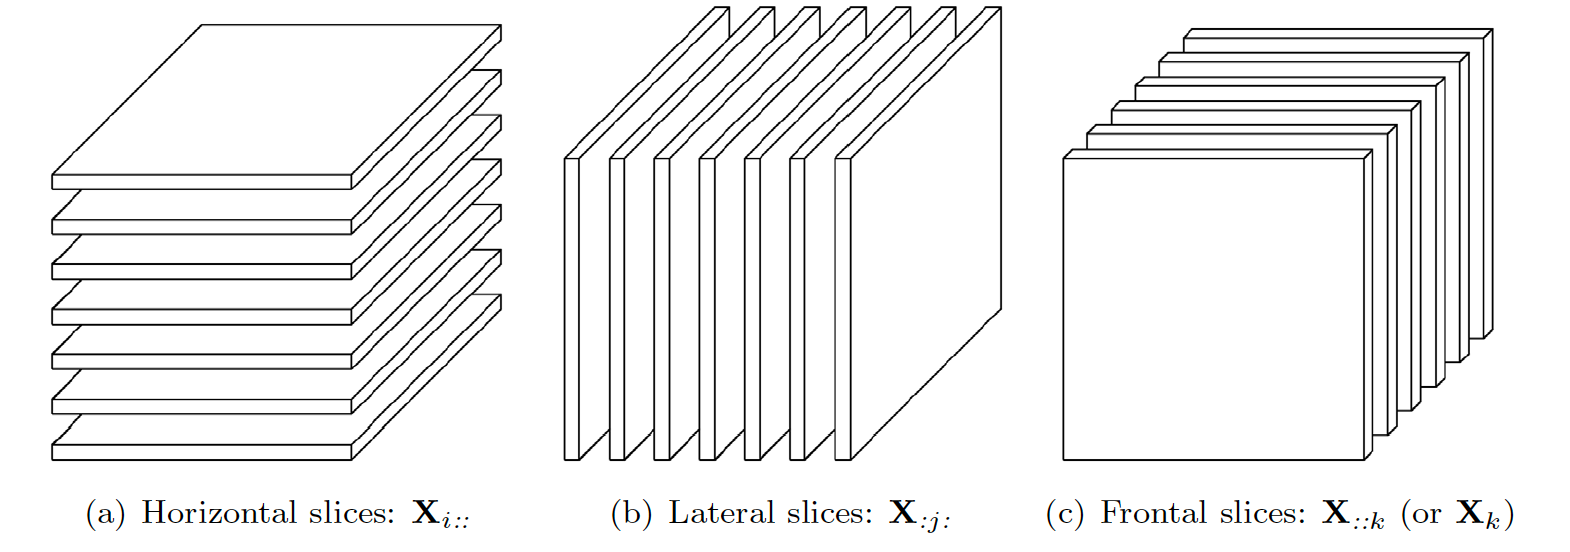
\includegraphics[keepaspectratio,width=4.8in, natwidth = 1570, natheight = 552]{figure/fig1.png}}
\caption{A visual representation of a third order tensor. It can be imagined in three distinct ways, depending on how you index it. This image is from \cite{tensors}}
\label{fig_ex1.png}
\end{figure}
%%%%%%%%%%%%%%%% end figure %%%%%%%%%%%%%%%%%%%
%%%%%%%%%%%%%%%% begin figure %%%%%%%%%%%%%%%%%%%
%%% 3.34in is the maximum width you can have for a figure
\begin{figure}
\center{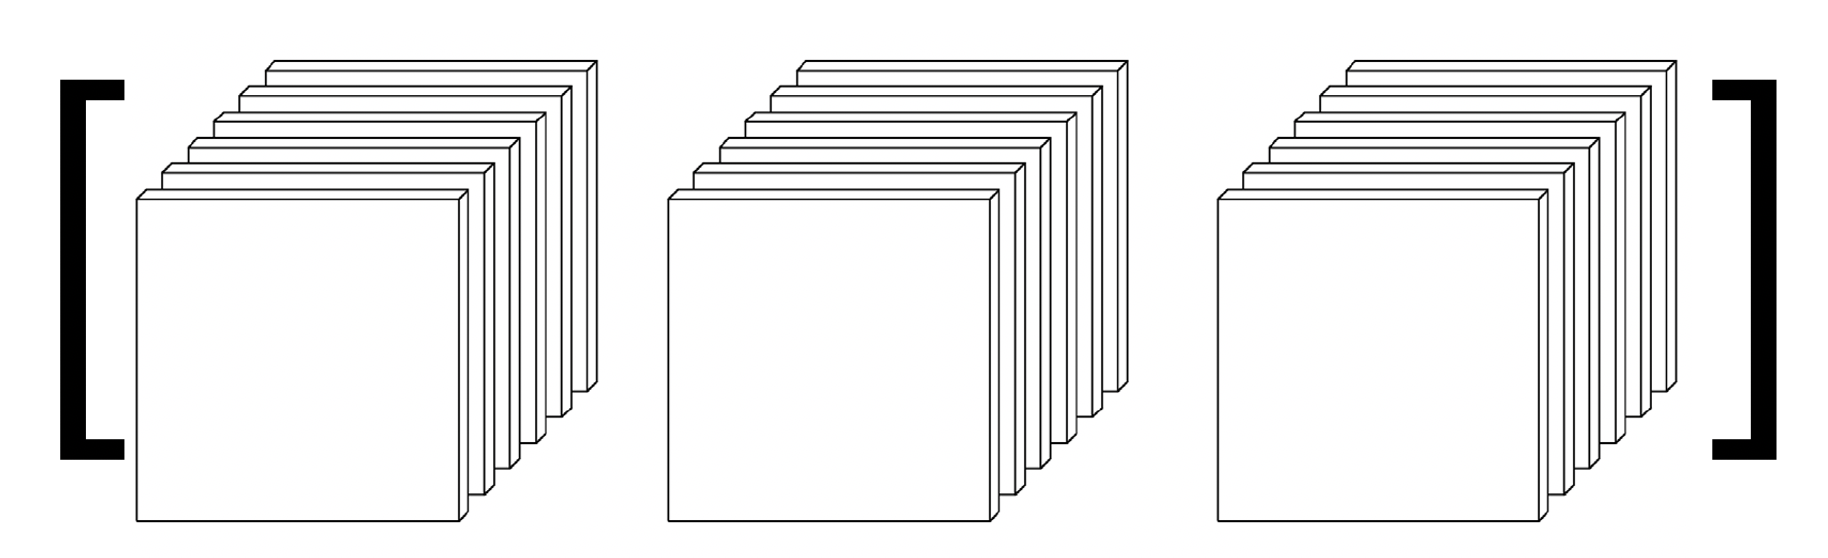
\includegraphics[keepaspectratio,width=4.8in, natwidth = 1828, natheight = 558]{figure/fig2.png}}
\caption{A visual representation of a fourth order tensor. In code, it is treated as a vector of third order tensors.}
\label{fig_ex2.png}
\end{figure}
%%%%%%%%%%%%%%%% end figure %%%%%%%%%%%%%%%%%%%

% %%%%%%%%%%%%%%%%%%%%%%%%%%%%%%%%%%%%%%%%%%%%%%%%%%%%%%%%%%%%%%%%%%%%%%
\section{An Overview of Tensors}

Before going into the details of how to implement reduced-order St. Venant-Kirchhoff deformable models, it's important to review tensors, as they show up in many places throughout this paper. The following explanation is influenced by \cite{tensors}, and contains extra findings that emerged through implementation.

A \textbf{tensor} is a multidimensional array. For example, a matrix is a second order tensor, and a vector is a first order tensor. An $N$th order tensor is an array of $N$ dimensions, and thus indexed using $N$ indices.

Figure~\ref{fig_ex1.png} shows a visual representation of a third order tensor; it can be imagined as a vector of matrices, where each square slice represents an individual matrix. Figure~\ref{fig_ex2.png} shows a visual representation of a fourth
order tensor, or a vector of third order tensors. Fourth order tensors are the highest dimension tensor needed for this paper, so no other tensor visuals are included.

There are three different kinds of tensor multiplication that we will use throughout this paper.

\subsection{Scalar Multiplication}

This works exactly as it seems like it would. For $a \in \mathbb{R}$, $\bm{X} \in \mathbb{R}^{I_1 \times I_2 \times ... \times I_N}$,

\begin{equation}
(a\bm{X})_{i_1, i_2, ..., i_n} = a\cdot x_{i_1, i_2, ..., i_n}
\end{equation}

%%%%%%%%%%%%%%%% begin figure %%%%%%%%%%%%%%%%%%%
%%% 3.34in is the maximum width you can have for a figure
\begin{figure}
\center{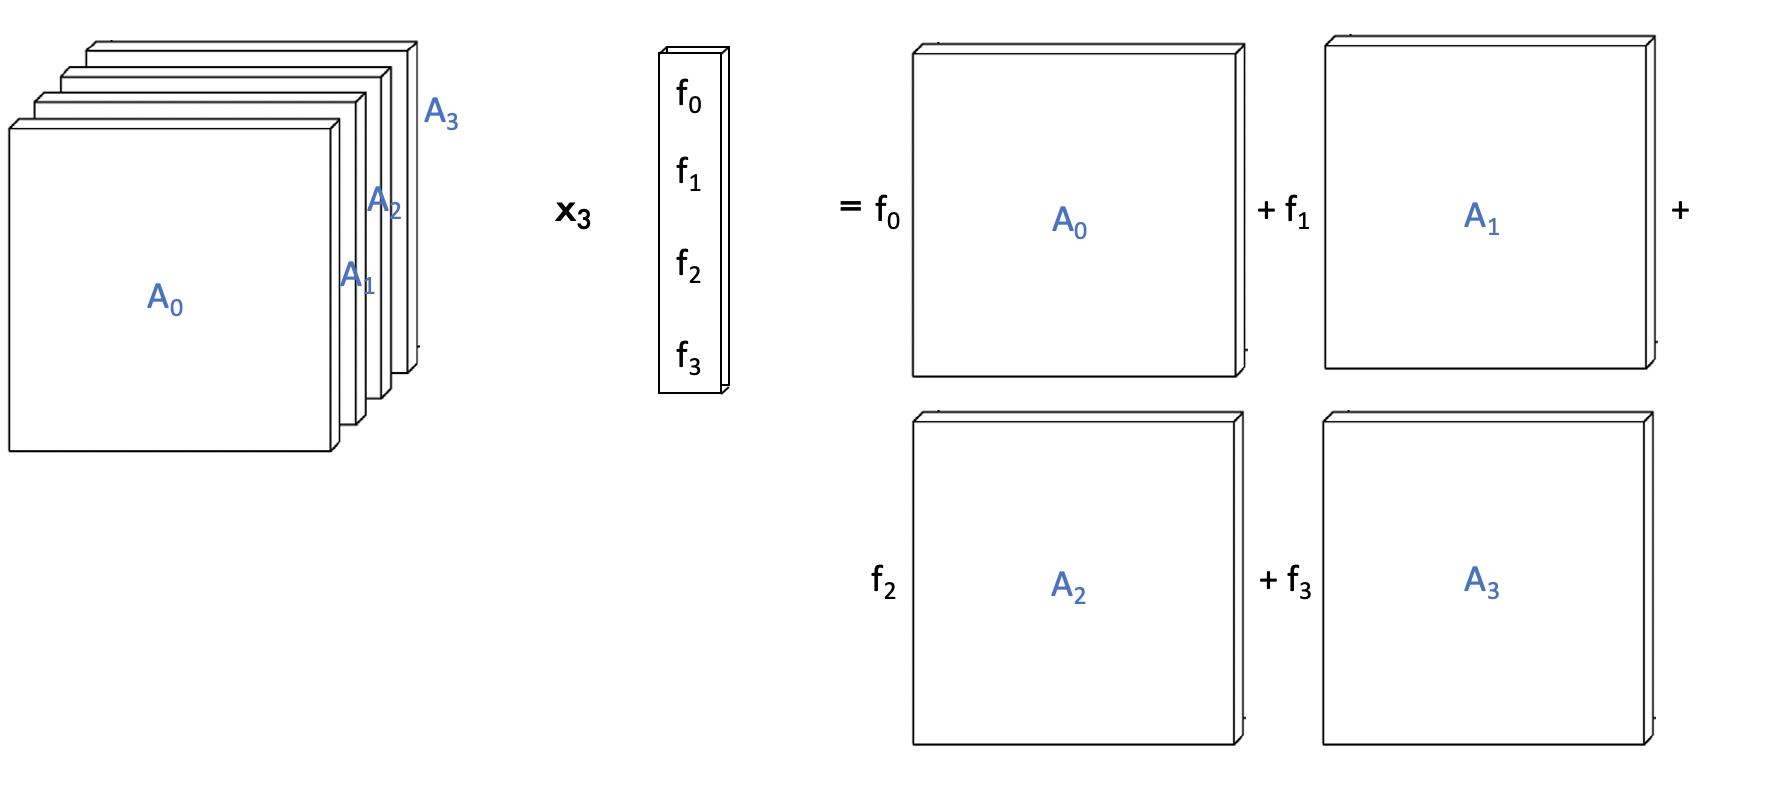
\includegraphics[keepaspectratio,width=4.8in, natwidth = 1774, natheight = 788]{figure/fig3.png}}
\caption{A visual representation of a 3-mode vector product, where $\bm{A} \in \mathbb{R}^{n \times n \times 4}$ and $\bm{f} \in \mathbb{R}^{4}$}
\label{fig_ex3.png}
\end{figure}
%%%%%%%%%%%%%%%% end figure %%%%%%%%%%%%%%%%%%%

\subsection{n-Mode Vector Product}

When a tensor is multiplied by a vector, its order reduces by 1. An n-mode vector product of a tensor $\bm{X} \in \mathbb{R}^{I_1 \times I_2 \times ... \times I_N}$ with a vector $\bm{v} \in \mathbb{R}^{I_n}$ is denoted by $\bm{X} \bar{\times}_n \bm{v}$. Element-wise,

\begin{equation}
(\bm{X} \bar{\times}_n \bm{v} )_{i_1, ..., i_{n-1}, i{n+1}, ..., i_N} = \sum_{i_n = 1}^{I_n} x_{i_1, i_2, ..., i_N}\cdot v_{i_n}
\end{equation}

So the resulting tensor $(\bm{X} \bar{\times}_n \bm{v} ) \in \mathbb{R}^{I_1 \times ... \times I_{n-1} \times I_{n+1} \times ... \times I_N}$. A visual representation of a 3-mode vector product can be seen in Figure~\ref{fig_ex3.png}.
For n-mode vector products, precedence matters, since it changes which dimension of the tensor is collapsed. Therefore, if $m < n$,

\begin{equation}
\bm{X} \bar{\times}_m \bm{a} \bar{\times}_n \bm{b} = (\bm{X} \bar{\times}_m \bm{a}) \bar{\times}_{n-1} \bm{b} = (\bm{X} \bar{\times}_n \bm{b}) \bar{\times}_m \bm{a}
\label{eq_vectorMode}
\end{equation}

This is an important rule that will be used later.

\subsection{n-Mode Matrix Product}
When a tensor is multiplied by a matrix, one of its dimensions changes. An n-mode matrix product of a tensor $\bm{X} \in \mathbb{R}^{I_1 \times I_2 \times ... \times I_N}$ with a matrix $\bm{U} \in \mathbb{R}^{J \times I_n}$ is denoted by $\bm{X} \times_n \bm{U}$. Element-wise, this multiplication results in:

\begin{equation}
(\bm{X} \times_n \bm{U} )_{i_1, ..., i_{n-1}, j, i{n+1}, ..., i_N} = \sum_{i_n = 1}^{I_n} x_{i_1, i_2, ..., i_N}\cdot u_{j,i_n}
\end{equation}

\noindent and the resulting tensor $(\bm{X} \times_n \bm{U} ) \in \mathbb{R}^{I_1 \times ... \times I_{n-1} \times J \times I_{n+1} \times ... \times I_N}$.

\bigskip
If $n \neq m$, then

\begin{equation}
\bm{X} \times_n \bm{A} \times_m  \bm{B} = \bm{X} \times_m \bm{B} \times_n \bm{A}
\label{eq_matrixModeCommute}
\end{equation}

If the modes are the same, then

\begin{equation}
\bm{X} \times_n \bm{A} \times_n  \bm{B} = \bm{X} \times_n (\bm{BA})
\label{eq_matrixModeAssociate}
\end{equation}

These two rules will also be used later. Another important rule which will be used later is, for  a tensor $\bm{X} \in \mathbb{R}^{I_1 \times I_2 \times ... \times I_N}$, a matrix $\bm{A} \in \mathbb{R}^{I_n, J}$, and a vector $\bm{b} \in \mathbb{R}^{J}$,

\begin{equation}
\bm{X} \bar{\times}_n (\bm{Ab}) = \bm{X} \times_n \bm{A^T} \bar{\times}_n \bm{b}
\label{eq_productDecompose}
\end{equation}

% %%%%%%%%%%%%%%%%%%%%%%%%%%%%%%%%%%%%%%%%%%%%%%%%%%%%%%%%%%%%%%%%%%%%%%
\section{Creating the Triangles}

When modeling solids using a discrete method, the model is represented by a mesh of polygons. In this paper, triangles were
used, so all results of this paper are based on triangle calculations.

In the code for this paper, a triangle object was created for cleaner implementation. Important variables to keep track of are:
\begin{enumerate}
  \item a vector of rest vertices. This should stay constant throughout the simulation.
  \item a vector of actual positions, which update as the whole mesh moves.
  \item a material model of some sort, to keep track of $\lambda$ and $\mu$ values for force calculations.
  \item rest area; this is used in calculating the internal force and stiffness matrix.
  \item precomputed coefficients for the cubic polynomial interpretation of internal force and quadratic polynomial
  for the tangent stiffness matrix. This will be discussed in a later section.
\end{enumerate}

In addition to storing variables, there are a few useful functions that can go into this object as well:
\begin{enumerate}
  \item getter/setter functions for all private variables.
  \item a function that computes $\frac{\partial \bm{F}}{\partial \bm{u}}$.
  \item a function that computes the deformation gradient, $\bm{F}$.
  \item a function to compute the internal force for the triangle given the deformation gradient.
  \item a function to compute the force Jacobian for the triangle given the deformation gradient.
\end{enumerate}

The last three functions are not necessary for the cubic polynomial approach, but are useful for debugging purposes.
All terms used in this section will be explained in the following subsections, which will go into more details of
implementation.

% %%%%%%%%%%%%%%%%%%%%%%%%%%%%%%%%%%%%%%%%%%%%%%%%%%%%%%%%%%%%%%%%%%%%%%
\subsection{Computing the Deformation Gradient}

When a solid is deformed, the \textbf{Deformation Gradient}, $\bm{F} \in \mathbb{R}^{2 \times 2}$, is the linear mapping from a rest vertex to its deformed position (without translation). This mapping can be used in the calculation of strain energy, so it's an important value to calculate if the cubic polynomial approach is not being used.

The deformation gradient can be found using the equation:

\begin{equation}
\bm{F} = \bm{D_sD_{m}^{-1}} = \begin{bmatrix} (x_2 - x_0) & (x_4 - x_0) \\ (x_3 - x_1) & (x_5 - x_1) \end{bmatrix} \bm{D_{m}^{-1}} = \begin{bmatrix} f_0 & f_2 \\ f_1 & f_3 \end{bmatrix}
\label{eq_F}
\end{equation}

\noindent where $\bm{D_s}$ is the spatial matrix made of the deformed vertices, $\bm{D_m}$ is the material matrix made of the rest vertices, and the three vertices of the triangle are $(x_0, x_1), (x_2, x_3), (x_4, x_5)$. Since the rest vertices stay constant throughout the simulation, $\bm{D_{m}^{-1}}$ is constant.

% %%%%%%%%%%%%%%%%%%%%%%%%%%%%%%%%%%%%%%%%%%%%%%%%%%%%%%%%%%%%%%%%%%%%%%
\subsection{Implementing StVK}

This section is not necessary for the cubic polynomial approach, but it's useful as a debugging tool. In the code
for this paper, the implementation of StVK is tied to the material of the triangle, and is called by the functions
that calculate internal force and the force Jacobian for an individual triangle.

A St. Venant-Kirchhoff deformable model is defined by the StVK strain energy, where

\begin{equation}
\psi = \mu ||\bm{F^TF} - \bm{I}||^2 + \frac{\lambda}{2}\tr (\bm{F^TF} - \bm{I})^2
\label{eq_stvk}
\end{equation}

\noindent and $\lambda$ and $\mu$ are Lamé coefficients.

In computing the internal force of a single triangle, the Piola-Kirchhoff stress tensor, i.e. the derivative of the strain energy by the deformation gradient, is used. The Piola-Kirchhoff stress tensor is

\begin{equation}
\frac{\partial \psi}{\partial \bm{F}} = 4\mu \bm{FF^TF} - 4\mu \bm{F} + 2\lambda \bm{F}\tr (\bm{F^TF}) -4\lambda \bm{F}
\label{eq_pk1}
\end{equation}

In computing the force Jacobian of a single triangle, the energy Hessian is used. The energy Hessian is:

\begin{equation}
  \begin{split}
\frac{\partial^2 \psi}{\partial \bm{F}^2} = 4\mu \left[\frac{\partial \bm{F}}{\partial F_i}\bm{F^TF} + \bm{F}\frac{\partial \bm{F}}{\partial F_i}^T\bm{F} + \bm{FF^T}\frac{\partial \bm{F}}{\partial F_i}\right] \\ + 2\lambda \frac{\partial \bm{F}}{\partial F_i}\tr \left(\bm{F^TF}\right) - 4[\mu + \lambda]\bm{I}
  \end{split}
\label{eq_dpdf}
\end{equation}

% %%%%%%%%%%%%%%%%%%%%%%%%%%%%%%%%%%%%%%%%%%%%%%%%%%%%%%%%%%%%%%%%%%%%%%
\subsection{Computing dF/dx}

Before we can calculate internal force and the force jacobian, we need to find the derivative of $\bm{F}$ in terms of $\bm{x}$. Remember that $\bm{F} \in \mathbb{R}^{2 \times 2}$ and $\bm{x} \in \mathbb{R}^6$. This means that

\begin{equation}
  \begin{split}
    \frac{\partial \bm{F}}{\partial \bm{x}} = \begin{bmatrix} \frac{\partial \bm{F}}{\partial x_0} & \frac{\partial \bm{F}}{\partial x_1}
    & \frac{\partial \bm{F}}{\partial x_2} & \frac{\partial \bm{F}}{\partial x_3} & \frac{\partial \bm{F}}{\partial x_4}
    & \frac{\partial \bm{F}}{\partial x_5} \end{bmatrix} \\ \\
    = \begin{bmatrix} \begin{bmatrix} -1 & -1 \\ 0 & 0 \end{bmatrix} & \begin{bmatrix} 0 & 0 \\ -1 & -1 \end{bmatrix}
  & \begin{bmatrix} 1 & 0 \\ 0 & 0 \end{bmatrix} & \begin{bmatrix} 0 & 0 \\ 1 & 0 \end{bmatrix}
  & \begin{bmatrix} 0 & 1 \\ 0 & 0 \end{bmatrix} & \begin{bmatrix} 0 & 0 \\ 0 & 1 \end{bmatrix}\end{bmatrix}
  \end{split}
\label{eq_dFdx}
\end{equation}

This was derived using equation~\ref{eq_F} for $\bm{F}$. Notice that this is a vector of matrices, i.e. a third order tensor. While we can use this as a third order tensor, it's easier to vectorize it and treat it as a matrix.

% %%%%%%%%%%%%%%%%%%%%%%%%%%%%%%%%%%%%%%%%%%%%%%%%%%%%%%%%%%%%%%%%%%%%%%
\subsubsection{Flattening Matrices and Tensors}

Flattening a tensor reduces it into a matrix, and flattening a matrix reduces it into a vector (also called vectorizing). To vectorize a matrix, we append the next column onto the bottom of the previous. So, as an example, if

\bigskip
\begin{center}
$\bm{A} = \begin{bmatrix} 1 & 3 \\ 2 & 4 \end{bmatrix}$
\end{center}

then

\begin{center}
$\vect (\bm{A}) = \begin{bmatrix} 1 \\ 2 \\ 3 \\ 4 \end{bmatrix}$
\end{center}

To flatten a tensor, we do this process on each level - so if we have a fourth order tensor, or a matrix of matrices, we first flatten the outer matrix into a vector of matrices, then vectorize the matrices inside. This step, which is the same for both third and fourth order tensors, can be done as shown below:

\bigskip
\begin{center}
$\bm{A} = \begin{bmatrix} \begin{bmatrix} 1 & 3 \\ 2 & 4 \end{bmatrix} & \begin{bmatrix} 5 & 7 \\ 6 & 8 \end{bmatrix} \end{bmatrix}$
\end{center}

then

\begin{center}
$\vect (\bm{A}) = \begin{bmatrix} \vect \left(\begin{bmatrix} 1 & 3 \\ 2 & 4 \end{bmatrix}\right) & \vect \left(\begin{bmatrix} 5 & 7 \\ 6 & 8 \end{bmatrix}\right) \end{bmatrix} = \begin{bmatrix} 1 & 5 \\ 2 & 6 \\ 3 & 7 \\ 4 & 8 \end{bmatrix}$
\end{center}

% %%%%%%%%%%%%%%%%%%%%%%%%%%%%%%%%%%%%%%%%%%%%%%%%%%%%%%%%%%%%%%%%%%%%%%
\subsection{Computing Internal Force and the Force Jacobian (The Non-Polynomial Way)}

This section is unnecessary for the cubic polynomial approach, but as with all the other sections, it's useful for debugging purposes. The internal force inside of the triangle can be computed using the equation

\begin{equation}
\bm{f} = \frac{\partial \psi}{\partial \bm{u}} = \vect \left(\frac{\partial \bm{F}}{\partial \bm{x}}\right)^T\cdot \vect \left(\frac{\partial \psi}{\partial \bm{F}}\right)
\label{eq_triforce}
\end{equation}

\noindent where the terms are defined by equations \ref{eq_dFdx} and \ref{eq_pk1}, respectively. The force Jacobian for each triangle can be computed using the equation

\begin{equation}
\frac{\partial^2 \psi}{\partial \bm{u}^2} = \vect \left(\frac{\partial \bm{F}}{\partial \bm{x}}\right)^T\cdot \frac{\partial^2 \psi}{\partial \bm{F}^2}\cdot \vect \left(\frac{\partial \bm{F}}{\partial \bm{x}}\right)
\label{eq_trijacob}
\end{equation}

\noindent where the terms are defined by equations \ref{eq_dFdx} and \ref{eq_dpdf}. Notice how $\bm{x}$, or current vertex placement, and $\bm{u}$, vertex \textit{displacement}, are used interchangeably here. In general, this is possible because the internal force at rest position $\bm{\bar{x}}$ is $0$, and $\bm{x} = \bm{\bar{x}} + \bm{u}$. However, it is important to note that these will \textbf{not} be interchangeable in the cubic polynomial approach.

% %%%%%%%%%%%%%%%%%%%%%%%%%%%%%%%%%%%%%%%%%%%%%%%%%%%%%%%%%%%%%%%%%%%%%%

\section{Creating the Triangle Mesh}

Now that a triangle object has been established, a triangle mesh can be built. In the code for this paper, the triangle mesh is a separate object from the individual triangles, and it stores all of the triangles in a vector. When constructing the triangle mesh, it may be useful to store a map of each vertex to its global position, so that future calculations are easier. In this implementation, the following were stored as private variables:

\begin{enumerate}
  \item a vector of triangles, i.e. the triangle mesh.
  \item a vertex to global index mapping.
  \item a vector of vertex placements.
  \item a vector of vertex rest positions.
  \item a vector of vertex displacements.
  \item a vector of vertex indices representing which vertices are \textbf{constrained}.
  \item a vector of vertex indices representing which vertices are \textbf{unconstrained}.
  \item a vector for internal force.
  \item a vector for external force.
  \item a mass matrix.
  \item a vector for velocity and a vector for acceleration.
  \item the basis reduction matrix.
  \item a vector for the reduced basis vector.
\end{enumerate}

% %%%%%%%%%%%%%%%%%%%%%%%%%%%%%%%%%%%%%%%%%%%%%%%%%%%%%%%%%%%%%%%%%%%%%%
\section{Implementing the Euler-Lagrange Equation of Motion}

After setting up the triangle mesh and applying some kind of external force, the system is animated by solving the Euler-Lagrange equation of motion. By solving equation~\ref{eq_motion}, the displacements for the next time step can be found and added to the vertex placements. In order to do this, each term of the equation must be calculated.

% %%%%%%%%%%%%%%%%%%%%%%%%%%%%%%%%%%%%%%%%%%%%%%%%%%%%%%%%%%%%%%%%%%%%%%
\subsection{Implementing Internal Force}

While this step is not necessary for the cubic polynomial approach, the methods are similar. In the previous section, the individual internal force for each triangle was calculated using equation~\ref{eq_triforce}. To calculate the global internal force, $\bm{R}(\bm{u}) \in \mathbb{R}^{2n}$, all of the individual internal forces are added up. This can be done by looping through every triangle, then looping through every vertex of the triangle. For each vertex, find where it belongs in the global context, and, if it is not constrained, add the force to the global vector. Here's an example through pseudocode below:

\bigskip
\begin{algorithmic}[1]
    \Function{globalInternalForce}{$null$}
        \State $global\_vector.setZero()$
        \For{triangle in triangles}
         \State $force \gets triangle.force()$
          \For{vertex in triangle vertices}
              \If {vertex is unconstrained}
                  \State $i \gets global\_index(vertex)$
                  \State add to global vector
              \EndIf
            \EndFor
        \EndFor
    \EndFunction
\end{algorithmic}

% %%%%%%%%%%%%%%%%%%%%%%%%%%%%%%%%%%%%%%%%%%%%%%%%%%%%%%%%%%%%%%%%%%%%%%
\subsection{Implementing the Tangent Stiffness Matrix}

The process here is similar to the process of calculating the global internal force. In the previous section, the individual force Jacobian for each triangle was calculated using equation~\ref{eq_trijacob}. To calculate the global stiffness matrix, $\bm{K}(\bm{u}) \in \mathbb{R}^{2n \times 2n}$, all of the individual force Jacobians are added up. This can be done by looping through every triangle, then looping through every vertex of the triangle twice. For each vertex, find where it belongs in the global context, and, if it is not constrained, add the force to the global stiffness matrix. Here's an example through pseudocode below:

\bigskip
\begin{algorithmic}[1]
    \Function{globalStiffnessMatrix}{$null$}
        \State $global\_stiffness.setZero()$
        \For{triangle in triangles}
         \State $jacobian \gets triangle.jacobian()$
          \For{$vertex$ in triangle vertices}
              \If {$vertex$ is unconstrained}
                  \State $i \gets global\_index(vertex)$
                  \For{$vertex_2$ in triangle vertices}
                      \If {$vertex_2$ is unconstrained}
                          \State $j \gets global\_index(vertex_2)$
                          \State add to global stiffness matrix
                      \EndIf
                    \EndFor
              \EndIf
            \EndFor
        \EndFor
    \EndFunction
\end{algorithmic}

% %%%%%%%%%%%%%%%%%%%%%%%%%%%%%%%%%%%%%%%%%%%%%%%%%%%%%%%%%%%%%%%%%%%%%%
\subsection{Implementing the Mass Matrix}

The mass matrix does not change over time, so this can be initialized outside of the motion function. How mass is implemented is up to the creator.

% %%%%%%%%%%%%%%%%%%%%%%%%%%%%%%%%%%%%%%%%%%%%%%%%%%%%%%%%%%%%%%%%%%%%%%
\subsection{Implementing the Damping Matrix}

The damping matrix is calculated using the equation

\begin{equation}
\bm{D}(\bm{u}) = \left(\alpha \bm{M} - \beta \bm{K}(\bm{u})\right)
\label{eq_damp}
\end{equation}

After computing the global stiffness matrix, this should be straightforward. The alpha and beta values are constant values that are up to the creator, depending on how strong the desired force is.

% %%%%%%%%%%%%%%%%%%%%%%%%%%%%%%%%%%%%%%%%%%%%%%%%%%%%%%%%%%%%%%%%%%%%%%
\subsection{Implementing the Newmark Integrator}

After calculating all of the individual terms in the Euler-Lagrange equation of motion, the equation can be solved for a given time-step using an implicit Newmark integrator. Implicit Newmark integrators are second-order accurate, and they only require one step, instead of having to solve the equation in a few iterations. While the pseudocode below is written for unreduced displacements, this iteration stays exactly the same when $\bm{u}$ is replaced with $\bm{q}$.

\bigskip
\begin{algorithmic}[1]
    \Function{NewmarkIntegrator}{$null$}
      \State $\bm{u_{i + 1}} \gets \bm{u_i}$
      \State Evaluate internal forces $\bm{R}(\bm{u_i})$
      \State Evaluate the stiffness matrix $\bm{K}(\bm{u_i})$
      \State Calculate the damping matrix, $\bm{D}(\bm{u_i}) = \alpha \bm{M} - \beta \bm{K}$
      \State Calculate the system matrix, $\bm{A} = \alpha_1\bm{M} + \alpha_4\bm{D}(\bm{u_i}) - \bm{K}$
      \State residual $\gets (\alpha_3\bm{M} - \alpha_6\bm{D}) \bm{ \ddot u_i} + (\alpha_2\bm{M} - \alpha_5\bm{D}) \bm{ \dot u_{i}} + \bm{R}(\bm{u_i}) + \bm{f_{i+1}}$
      \State $ \Delta \bm{u} \gets \bm{A^{-1}} \cdot $ residual
      \State $ \bm{u_{i + 1}} \gets \bm{u_{i + 1}} + \Delta \bm{u}$
      \State $ \bm{ \dot u_{i + 1}} \gets \alpha_4(\bm{u_{i+1}} - \bm{u_i}) + \alpha_5 \bm{ \dot u_i} + \alpha_6 \bm{ \ddot u_i}$
      \State $ \bm{ \ddot u_{i + 1}} \gets \alpha_1(\bm{u_{i+1}} - \bm{u_i}) - \alpha_2 \bm{\dot u_i} - \alpha_3 \bm{\ddot u_i}$
    \EndFunction
\end{algorithmic}

\bigskip
The alpha constants in this integrator are determined by the equations

\begin{center}
$\alpha_1 = \frac{1}{\tilde{\beta}(\Delta t)^2}, \alpha_2 = \frac{1}{\tilde{\beta}\Delta t},
\alpha_3 = \frac{1 - 2\tilde{\beta}}{2\tilde{\beta}}, \alpha_4 = \frac{\tilde{\gamma}}{\tilde{\beta}\Delta t},$

$\alpha_5 = 1 - \frac{\tilde{\gamma}}{\tilde{\beta}}, \alpha_6 = \left(1 - \frac{\tilde{\gamma}}{2\tilde{\beta}}\right)\Delta t$
\end{center}

Where $0 \leq \tilde{\beta} \leq 0.5$ and $0 \leq \tilde{\gamma} \leq 1$. We chose $\tilde{\beta} = 0.25$ and $\tilde{\gamma} = 0.5$ for this implementation, but Barbič and James chose $\tilde{\beta} = 0$ and $\tilde{\gamma} = 0.5$.

% %%%%%%%%%%%%%%%%%%%%%%%%%%%%%%%%%%%%%%%%%%%%%%%%%%%%%%%%%%%%%%%%%%%%%%
\section{Generating Precomputed Coefficients}

At this point in the paper, a fully function simulator of St. Venant-Kirchhoff deformable models can be created; however, they are still unreduced and lack any pre-computation. If pre-computation does not interest you, feel free to skip to the section titled \textbf{Generating a Deformation Basis} - after creating a deformation basis, reducing everything is as simple as following equations \ref{eq_basisreduction} - \ref{eq_rstiffness}.

For simplicity, we derived the precomputed constant coefficients before reducing the equation. In order to have the ability to precompute constant coefficients, all variables must be extractable. In the case of unreduced St. Venant-Kirchhoff models, this means that we should be able to separate vertex positions, $\bm{x}$, out of the internal force and stiffness matrix calculation. Again, for simplicity, we began by separating $\bm{x}$ from the internal force equation \ref{eq_triforce} and force Jacobian equation \ref{eq_trijacob} for an individual triangle, then created global constants similar to how the global internal force and global stiffness matrix were built in sections 5.1 and 5.2.

% %%%%%%%%%%%%%%%%%%%%%%%%%%%%%%%%%%%%%%%%%%%%%%%%%%%%%%%%%%%%%%%%%%%%%%
\subsection{Coefficients for the Tangent Stiffness Matrix}

Looking at equation~\ref{eq_dpdf}, there is clearly one quadratic term, and one constant matrix, $-4[\mu + \lambda]\bm{I}$. From this, we can already derive the constant coefficient term:

\begin{equation}
  \bm{Q} = - \vect \left(\frac{\partial \bm{F}}{\partial \bm{x}}\right)^T 4[\mu + \lambda]\bm{I} \vect \left(\frac{\partial \bm{F}}{\partial \bm{x}}\right)
  \label{eq_unreducedConst}
\end{equation}

The quadratic term is trickier. Looking at the $\mu$ term of $\frac{\partial^2 \psi}{\partial \bm{F}^2}$ alone, $\left[\frac{\partial \bm{F}}{\partial F_i}\bm{F^TF} + \bm{F}\frac{\partial \bm{F}}{\partial F_i}^T\bm{F} + \bm{FF^T}\frac{\partial \bm{F}}{\partial F_i}\right]$ decomposes into

\begin{center}
$\frac{\partial \bm{F}}{\partial F_i}\bm{F^TF} = \begin{bmatrix} f_{0}^2 + f_{1}^2 & 0 & f_0f_2 + f_1f_3 & 0 \\
0 & f_{0}^2 + f_{1}^2 & 0 & f_0f_2 + f_1f_3 \\
f_0f_2 + f_1f_3 & 0 & f_{2}^2 + f_{3}^2 & 0 \\
0 & f_0f_2 + f_1f_3 & 0 & f_{2}^2 + f_{3}^2 \end{bmatrix}$

\bigskip
$\bm{F}\frac{\partial \bm{F}}{\partial F_i}^T\bm{F} = \begin{bmatrix} f_{0}^2 & f_0f_1 & f_0f_2 & f_1f_2  \\
f_0f_1 & f_{1}^2 & f_0f_3 & f_1f_3 \\
f_0f_2 & f_0f_3 & f_{2}^2 & f_2f_3 \\
f_1f_2 & f_1f_3 & f_2f_3 & f_{3}^2 \end{bmatrix}$

\bigskip
$\bm{FF^T}\frac{\partial \bm{F}}{\partial F_i} = \begin{bmatrix} f_{0}^2 + f_{2}^2 & f_0f_1 + f_2f_3 & 0 & 0  \\
f_0f_1 + f_2f_3 & f_{1}^2 + f_{3}^2 & 0 & 0 \\
0 & 0 & f_{0}^2 + f_{2}^2 & f_0f_1 + f_2f_3 \\
0 & 0 & f_0f_1 + f_2f_3 & f_{1}^2 + f_{3}^2 \end{bmatrix}$
\end{center}

In order to separate out all of the $\bm{x}$'s, we can first separate all of the $\bm{f}$ terms. This can be done using tensors. By working backwards from the matrices above, a fourth order tensor, $\bm{C_{\mu}}$, can be derived, such that

\begin{equation}
    \bm{C_{\mu}} = \begin{bmatrix}
    \begin{bmatrix} 3 & 0 & 0 & 0 \\ 0 & 1 & 0 & 0 \\ 0 & 0 & 1 & 0 \\ 0 & 0 & 0 & 0 \end{bmatrix} &
    \begin{bmatrix} 0 & 2 & 0 & 0 \\ 0 & 0 & 0 & 0 \\ 0 & 0 & 0 & 1 \\ 0 & 0 & 0 & 0 \end{bmatrix} &
    \begin{bmatrix} 0 & 0 & 2 & 0 \\ 0 & 0 & 0 & 1 \\ 0 & 0 & 0 & 0 \\ 0 & 0 & 0 & 0 \end{bmatrix} &
    \begin{bmatrix}0 & 0 & 0 & 0 \\ 0 & 0 & 0 & 0 \\ 0 & 1 & 0 & 0 \\ 0 & 0 & 0 & 0 \end{bmatrix} \\
      \begin{bmatrix} 0 & 0 & 0 & 0 \\ 2 & 0 & 0 & 0 \\ 0 & 0 & 0 & 0 \\ 0 & 0 & 1 & 0 \end{bmatrix} &
      \begin{bmatrix} 1 & 0 & 0 & 0 \\ 0 & 3 & 0 & 0 \\ 0 & 0 & 0 & 0 \\ 0 & 0 & 0 & 1 \end{bmatrix} &
      \begin{bmatrix} 0 & 0 & 0 & 0 \\ 0 & 0 & 0 & 0 \\ 0 & 0 & 0 & 0 \\ 1 & 0 & 0 & 0 \end{bmatrix} &
      \begin{bmatrix}0 & 0 & 1 & 0 \\ 0 & 0 & 0 & 2 \\ 0 & 0 & 0 & 0 \\ 0 & 0 & 0 & 0 \end{bmatrix} \\
        \begin{bmatrix} 0 & 0 & 0 & 0 \\ 0 & 0 & 0 & 0 \\ 2 & 0 & 0 & 0 \\ 0 & 1 & 0 & 0 \end{bmatrix} &
        \begin{bmatrix} 0 & 0 & 0 & 1 \\ 0 & 0 & 0 & 0 \\ 0 & 0 & 0 & 0 \\ 0 & 0 & 0 & 0 \end{bmatrix} &
        \begin{bmatrix} 1 & 0 & 0 & 0 \\ 0 & 0 & 0 & 0 \\ 0 & 0 & 3 & 0 \\ 0 & 0 & 0 & 1 \end{bmatrix} &
        \begin{bmatrix}0 & 1 & 0 & 0 \\ 0 & 0 & 0 & 0 \\ 0 & 0 & 0 & 2 \\ 0 & 0 & 0 & 0 \end{bmatrix} \\
          \begin{bmatrix} 0 & 0 & 0 & 0 \\ 0 & 0 & 1 & 0 \\ 0 & 0 & 0 & 0 \\ 0 & 0 & 0 & 0 \end{bmatrix} &
          \begin{bmatrix} 0 & 0 & 0 & 0 \\ 0 & 0 & 0 & 0 \\ 1 & 0 & 0 & 0 \\ 0 & 2 & 0 & 0 \end{bmatrix} &
          \begin{bmatrix} 0 & 0 & 0 & 0 \\ 1 & 0 & 0 & 0 \\ 0 & 0 & 0 & 0 \\ 0 & 0 & 2 & 0 \end{bmatrix} &
          \begin{bmatrix}0 & 0 & 0 & 0 \\ 0 & 1 & 0 & 0 \\ 0 & 0 & 1 & 0 \\ 0 & 0 & 0 & 3 \end{bmatrix} \end{bmatrix}
\label{_eq_quadmu}
\end{equation}

And
\begin{equation}
\begin{split}
4\mu\left[\frac{\partial \bm{F}}{\partial F_i}\bm{F^TF} + \bm{F}\frac{\partial \bm{F}}{\partial F_i}^T\bm{F} + \bm{FF^T}\frac{\partial \bm{F}}{\partial F_i}\right] =
\\ 4\mu \bm{C_{\mu}} \bar{\times}_4 \vect (\bm{F}) \bar{\times}_3 \vect (\bm{F})
\end{split}
\end{equation}

Similar to the $\mu$ term, the $\lambda$ term, which can be split into the two terms:

\begin{center}
  $2\lambda \left(\frac{\partial \bm{F}}{\partial F_i}\tr \left(\bm{F^TF}\right) \right)  = 2\lambda \left(f_{0}^2 + f_{1}^2 + f_{2}^2  + f_{3}^2\right) \begin{bmatrix}
  1 & 0 & 0 & 0  \\
  0 & 1  & 0 & 0 \\
  0 & 0 & 1  & 0 \\
  0 & 0 & 0 & 1  \end{bmatrix}$

  \bigskip
  $2\lambda \left(\bm{F}\frac{\partial \tr \left(\bm{F^TF}\right)}{\partial F_i}\right)  = 2\lambda \begin{bmatrix}
  2f_{0}^2 & 2f_0f_1 & 2f_0f_2 & 2f_0f_3  \\
  2f_0f_1 & 2f_{1}^2 & 2f_1f_2 & 2f_1f_3 \\
  2f_0f_2 & 2f_1f_2 & 2f_{2}^2 & 2f_2f_3 \\
  2f_0f_3 & 2f_1f_3 & 2f_2f_3 & 2f_{3}^2  \end{bmatrix}$
\end{center}

has a fourth order tensors that can be derived:

\begin{equation}
    \bm{C_{\lambda}} = \begin{bmatrix}
    \begin{bmatrix} 3 & 0 & 0 & 0 \\ 0 & 1 & 0 & 0 \\ 0 & 0 & 1 & 0 \\ 0 & 0 & 0 & 1 \end{bmatrix} &
    \begin{bmatrix} 0 & 2 & 0 & 0 \\ 2 & 0 & 0 & 0 \\ 0 & 0 & 0 & 0 \\ 0 & 0 & 0 & 0 \end{bmatrix} &
    \begin{bmatrix} 0 & 0 & 2 & 0 \\ 0 & 0 & 0 & 0 \\ 2 & 0 & 0 & 0 \\ 0 & 0 & 0 & 0 \end{bmatrix} &
    \begin{bmatrix}0 & 0 & 0 & 2 \\ 0 & 0 & 0 & 0 \\ 0 & 0 & 0 & 0 \\ 2 & 0 & 0 & 0 \end{bmatrix} \\
      \begin{bmatrix} 0 & 0 & 0 & 0 \\ 0 & 0 & 0 & 0 \\ 0 & 0 & 0 & 0 \\ 0 & 0 & 0 & 0 \end{bmatrix} &
      \begin{bmatrix} 1 & 0 & 0 & 0 \\ 0 & 3 & 0 & 0 \\ 0 & 0 & 1 & 0 \\ 0 & 0 & 0 & 1 \end{bmatrix} &
      \begin{bmatrix} 0 & 0 & 0 & 0 \\ 0 & 0 & 2 & 0 \\ 0 & 2 & 0 & 0 \\ 0 & 0 & 0 & 0 \end{bmatrix} &
      \begin{bmatrix}0 & 0 & 0 & 0 \\ 0 & 0 & 0 & 2 \\ 0 & 0 & 0 & 0 \\ 0 & 2 & 0 & 0 \end{bmatrix} \\
        \begin{bmatrix} 0 & 0 & 0 & 0 \\ 0 & 0 & 0 & 0 \\ 0 & 0 & 0 & 0 \\ 0 & 0 & 0 & 0 \end{bmatrix} &
        \begin{bmatrix} 0 & 0 & 0 & 0 \\ 0 & 0 & 0 & 0 \\ 0 & 0 & 0 & 0 \\ 0 & 0 & 0 & 0 \end{bmatrix} &
        \begin{bmatrix} 1 & 0 & 0 & 0 \\ 0 & 1 & 0 & 0 \\ 0 & 0 & 3 & 0 \\ 0 & 0 & 0 & 1 \end{bmatrix} &
        \begin{bmatrix}0 & 0 & 0 & 0 \\ 0 & 0 & 0 & 0 \\ 0 & 0 & 0 & 2 \\ 0 & 0 & 2 & 0 \end{bmatrix} \\
          \begin{bmatrix} 0 & 0 & 0 & 0 \\ 0 & 0 & 0 & 0 \\ 0 & 0 & 0 & 0 \\ 0 & 0 & 0 & 0 \end{bmatrix} &
          \begin{bmatrix} 0 & 0 & 0 & 0 \\ 0 & 0 & 0 & 0 \\ 0 & 0 & 0 & 0 \\ 0 & 0 & 0 & 0 \end{bmatrix} &
          \begin{bmatrix} 0 & 0 & 0 & 0 \\ 0 & 0 & 0 & 0 \\ 0 & 0 & 0 & 0 \\ 0 & 0 & 0 & 0 \end{bmatrix} &
          \begin{bmatrix}1 & 0 & 0 & 0 \\ 0 & 1 & 0 & 0 \\ 0 & 0 & 1 & 0 \\ 0 & 0 & 0 & 3 \end{bmatrix} \end{bmatrix}
\label{_eq_quadlambda}
\end{equation}

And
\begin{equation}
2\lambda \left[\frac{\partial \bm{F}}{\partial F_i}\tr \left(\bm{F^TF}\right) + \bm{F}\frac{\partial \tr \left(\bm{F^TF}\right)}{\partial F_i} \right] = 2\lambda \bm{C_{\lambda}} \bar{\times}_4 \vect (\bm{F}) \bar{\times}_3 \vect (\bm{F})
\end{equation}

So the entire quadratic term of equation~\ref{eq_dpdf} can be written as

\begin{multline}
\bm{C_f} \bar{\times}_4 \vect (\bm{F}) \bar{\times}_3 \vect (\bm{F}) =  \\ \left(4\mu \bm{C_{\mu}} + 2\lambda \bm{C_{\lambda}}\right) \bar{\times}_4 \vect (\bm{F}) \bar{\times}_3 \vect (\bm{F})
\end{multline}

This still only separates $\bm{F}$, not $\bm{x}$. However, since $\bm{F} = \frac{\partial \bm{F}}{\partial \bm{x}}\bm{x}$, we can rearrange this equation using our tensor product rules (equations~\ref{eq_vectorMode}-\ref{eq_productDecompose}) so that
\begin{center}
  \begin{multline}
  \bm{C_f} \bar{\times}_4 \vect (\bm{F}) \bar{\times}_3 \vect (\bm{F}) = \bm{C_f} \bar{\times}_4 \vect \left( \frac{\partial \bm{F}}{\partial \bm{x}}\bm{x}\right) \bar{\times}_3 \vect \left( \frac{\partial \bm{F}}{\partial \bm{x}}\bm{x}\right)
  \\ = \bm{C_f} \bar{\times}_4 \vect \left( \frac{\partial \bm{F}}{\partial \bm{x}}\right) \vect (\bm{x}) \bar{\times}_3 \vect \left( \frac{\partial \bm{F}}{\partial \bm{x}}\right) \vect (\bm{x})
  \\ = \bm{C_f} \times_4 \vect \left( \frac{\partial \bm{F}}{\partial \bm{x}}\right)^T \bar{\times}_4 \vect (\bm{x}) \times_3 \vect \left( \frac{\partial \bm{F}}{\partial \bm{x}}\right)^T \bar{\times}_3 \vect (\bm{x})
  \\ = \left[\bm{C_f} \times_4 \vect \left( \frac{\partial \bm{F}}{\partial \bm{x}}\right)^T \times_3 \vect \left( \frac{\partial \bm{F}}{\partial \bm{x}}\right)^T\right] \bar{\times}_4 \vect (\bm{x}) \bar{\times}_3 \vect (\bm{x})
\end{multline}
\end{center}

Since $\frac{\partial \bm{F}}{\partial \bm{x}}$ is constant (refer back to equation~\ref{eq_dFdx}), this can be pushed into our constant, so that our equation~\ref{eq_dpdf} quadratic constant can be written as

\begin{equation}
\bm{C_{dpdf}}  = \bm{C_f} \times_4 \vect \left( \frac{\partial \bm{F}}{\partial \bm{x}} \right)^T \times_3 \vect \left( \frac{\partial \bm{F}}{\partial \bm{x}}\right)^T
\end{equation}

This constant is still for equation~\ref{eq_dpdf}, not the force Jacobian. The only step left in calculating the triangle force Jacobian's quadratic coefficient is to multiply it on both sides by $\left(\frac{\partial \bm{F}}{\partial \bm{x}}\right)$:

\begin{multline}
\bm{C}  = \vect \left( \frac{\partial \bm{F}}{\partial \bm{x}} \right)^T \bm{C_{dpdf}} \vect \left( \frac{\partial \bm{F}}{\partial \bm{x}} \right)
\\ = \bm{C_{dpdf}} \times_2 \vect \left( \frac{\partial \bm{F}}{\partial \bm{x}} \right)^T \times_1 \vect \left( \frac{\partial \bm{F}}{\partial \bm{x}}\right)^T
\end{multline}

With both the quadratic coefficient and the constant matrix, the force jacobian can now be written as a quadratic polynomial:

\begin{equation}
\frac{\partial^2 \psi}{\partial \bm{x}^2} = \bm{C} \bar{\times}_4 \vect (\bm{x}) \bar{\times}_3 \vect (\bm{x}) + \bm{Q}
\label{eq_unreducedQuadratic}
\end{equation}

% %%%%%%%%%%%%%%%%%%%%%%%%%%%%%%%%%%%%%%%%%%%%%%%%%%%%%%%%%%%%%%%%%%%%%%
\subsubsection{Creating the Global Tangent Stiffness Matrix Coefficients}

Now that the constant terms for the force Jacobian for each triangle have been computed, we can create global constant terms for the tangent stiffness matrix in a similar manner to how the global tangent stiffness matrix was computed earlier.

\bigskip
\begin{algorithmic}[1]
    \Function{globalStiffnessConstants}{$null$}
        \State $Q_{global}.setZero()$
        \State $C_{global}.setZero()$
        \For{triangle in triangles}
         \State $Q \gets triangle.getQ()$
         \State $C \gets triangle.getC()$
          \For{$vertex$ in triangle vertices}
              \If {$vertex$ is unconstrained}
                  \State $i \gets global\_index(vertex)$
                  \For{$vertex_2$ in triangle vertices}
                      \If {$vertex_2$ is unconstrained}
                          \State $j \gets global\_index(vertex_2)$
                          \State $Q_{global}(i,j) \gets Q_{global}(i,j) + Q(vertex, vertex_2)$
                          \For{$vertex_3$ in triangle vertices}
                                \State $k \gets global\_index(vertex_3)$
                                \For{$vertex_4$ in triangle vertices}
                                    \State $l \gets global\_index(vertex_4)$
                                    \State $C_{global}(i,j,k,l)  \gets C_{global}(i,j,k,l)+C(vertex, vertex_2, vertex_3, vertex_4)$
                                  \EndFor
                            \EndFor
                      \EndIf
                    \EndFor
              \EndIf
            \EndFor
        \EndFor
    \EndFunction
\end{algorithmic}

Note that the global coefficients match the order of the triangle coefficients; that is, the constant term, $\bm{Q_{global}}$, is a matrix, while the global coefficient for the quadratic term, $\bm{C_{global}}$, is a fourth-order tensor. The difference is in their dimensions; while $\bm{Q} \in \mathbb{R}^{6 \times 6}$, $\bm{Q_{global}} \in \mathbb{R}^{2n \times 2n}$, and while  $\bm{C} \in \mathbb{R}^{6 \times 6 \times 6 \times 6}$, $\bm{C_{global}} \in \mathbb{R}^{2n \times 2n \times 2n \times 2n}$.

Also note that this pseudocode is abbreviated; while it only shows adding $\bm{C}$ and $\bm{Q}$ to one position in the global coefficients, you actually have to add it to every possible combination of the current vertices' $x$ and $y$ coordinates. For example, if $vertex$ and $vertex_2$ are unconstrained, then

\begin{center}
$\bm{Q_{global}}(i,j) += \bm{Q}(vertex(x), vertex_2(x))$,

$\bm{Q_{global}}(i + 1,j) += \bm{Q}(vertex(y), vertex_2(x))$,

$\bm{Q_{global}}(i ,j + 1) += \bm{Q}(vertex(x), vertex_2(y))$, and

$\bm{Q_{global}}(i + 1,j + 1) += \bm{Q}(vertex(y), vertex_2(y))$.
\end{center}

After all coefficients are precomputed, the global stiffness matrix calculation is as easy as computing:

\begin{equation}
  \bm{K}(\bm{x}) = \bm{C_{global}} \bar{\times}_4 \bm{x} \bar{\times}_3 \bm{x} + \bm{Q_{global}}
\end{equation}

% %%%%%%%%%%%%%%%%%%%%%%%%%%%%%%%%%%%%%%%%%%%%%%%%%%%%%%%%%%%%%%%%%%%%%%
\subsection{Coefficients for Internal Force}

Looking at equation~\ref{eq_pk1}, there is clearly one cubic term and one linear term. Since the force Jacobian is the derivative of internal force, the linear coefficient for internal force is actually also $\bm{Q}$ (eq \ref{eq_unreducedConst}). The connection between the cubic term and the quadratic term, however, is not as clean, because the cubic term can be reduced into a fourth order tensor as well. We are able to reduce the coefficient for the cubic term into a fourth order tensor because equation~\ref{eq_pk1} is vectorized, reducing its order by one.

The vectorized cubic term, before separating $\bm{x}$, is

\begin{center}
  $\vect \left( 4\mu\bm{FF^TF} + 2\lambda\tr\left(\bm{F^TF}\right)\bm{F}\right)$
\end{center}

where

\begin{center}
  $\vect \left( 4\mu\bm{FF^TF} \right) = 4\mu
  \begin{bmatrix}
    f_{0}^3 + f_0f_{1}^2 + f_0f_{2}^2 + f_1f_2f_3 \\
    f_{0}^2f_{1} + f_{1}^3 + f_0f_2f_3 + f_1f_{3}^2 \\
    f_{0}^2f_{2} + f_0f_1f_3 + f_{2}^3 + f_2f_{3}^2 \\
    f_0f_1f_2 + f_{1}^2f_3 + f_{2}^2f_3 + f_{3}^3 \\
    \end{bmatrix}$

    \bigskip
    $\vect \left( 2\lambda\tr\left(\bm{F^TF}\right)\bm{F} \right) = 2\lambda
    \begin{bmatrix}
      f_{0}^3 + f_0f_{1}^2 + f_0f_{2}^2 + f_0f_{3}^2 \\
      f_{0}^2f_1 + f_{1}^3 + f_1f_{2}^2 + f_1f_{3}^2 \\
      f_{0}^2f_2 + f_2f_{1}^2 + f_{2}^3 + f_2f_{3}^2 \\
      f_{0}^2f_3 + f_3f_{1}^2 + f_3f_{2}^2 + f_{3}^3\\
      \end{bmatrix}$
\end{center}

In order to separate out all of the $\bm{x}$'s, we can first separate all of the $\bm{f}$ terms, like we did for the force jacobian. By working backwards from the matrices above, two fourth order tensor, $\bm{A_{\mu}}$ and $\bm{A_{\lambda}}$, can be derived, such that

\begin{equation}
    \bm{A_{\mu}} = \begin{bmatrix}
    \begin{bmatrix} 1 & 0 & 0 & 0 \\ 0 & 1 & 0 & 0 \\ 0 & 0 & 1 & 0 \\ 0 & 0 & 0 & 0 \end{bmatrix} &
    \begin{bmatrix} 0 & 0 & 0 & 0 \\ 0 & 0 & 0 & 0 \\ 0 & 0 & 0 & 1 \\ 0 & 0 & 0 & 0 \end{bmatrix} &
    \begin{bmatrix} 0 & 0 & 0 & 0 \\ 0 & 0 & 0 & 0 \\ 0 & 0 & 0 & 0 \\ 0 & 0 & 0 & 0 \end{bmatrix} &
    \begin{bmatrix} 0 & 0 & 0 & 0 \\ 0 & 0 & 0 & 0 \\ 0 & 0 & 0 & 0 \\ 0 & 0 & 0 & 0 \end{bmatrix} \\
      \begin{bmatrix} 0 & 0 & 0 & 0 \\ 0 & 0 & 0 & 0 \\ 0 & 0 & 0 & 0 \\ 0 & 0 & 1 & 0 \end{bmatrix} &
      \begin{bmatrix} 1 & 0 & 0 & 0 \\ 0 & 1 & 0 & 0 \\ 0 & 0 & 0 & 0 \\ 0 & 0 & 0 & 1 \end{bmatrix} &
      \begin{bmatrix} 0 & 0 & 0 & 0 \\ 0 & 0 & 0 & 0 \\ 0 & 0 & 0 & 0 \\ 0 & 0 & 0 & 0 \end{bmatrix} &
      \begin{bmatrix} 0 & 0 & 0 & 0 \\ 0 & 0 & 0 & 0 \\ 0 & 0 & 0 & 0 \\ 0 & 0 & 0 & 0 \end{bmatrix} \\
        \begin{bmatrix} 0 & 0 & 0 & 0 \\ 0 & 0 & 0 & 0 \\ 0 & 0 & 0 & 0 \\ 0 & 0 & 0 & 0 \end{bmatrix} &
        \begin{bmatrix} 0 & 0 & 0 & 0 \\ 0 & 0 & 0 & 0 \\ 0 & 0 & 0 & 0 \\ 0 & 0 & 0 & 0 \end{bmatrix} &
        \begin{bmatrix} 1 & 0 & 0 & 0 \\ 0 & 0 & 0 & 0 \\ 0 & 0 & 1 & 0 \\ 0 & 0 & 0 & 1 \end{bmatrix} &
        \begin{bmatrix} 0 & 1 & 0 & 0 \\ 0 & 0 & 0 & 0 \\ 0 & 0 & 0 & 0 \\ 0 & 0 & 0 & 0 \end{bmatrix} \\
          \begin{bmatrix} 0 & 0 & 0 & 0 \\ 0 & 0 & 0 & 0 \\ 0 & 0 & 0 & 0 \\ 0 & 0 & 0 & 0 \end{bmatrix} &
          \begin{bmatrix} 0 & 0 & 0 & 0 \\ 0 & 0 & 0 & 0 \\ 0 & 0 & 0 & 0 \\ 0 & 0 & 0 & 0 \end{bmatrix} &
          \begin{bmatrix} 0 & 0 & 0 & 0 \\ 1 & 0 & 0 & 0 \\ 0 & 0 & 0 & 0 \\ 0 & 0 & 0 & 0 \end{bmatrix} &
          \begin{bmatrix} 0 & 0 & 0 & 0 \\ 0 & 1 & 0 & 0 \\ 0 & 0 & 1 & 0 \\ 0 & 0 & 0 & 1 \end{bmatrix} \\ \end{bmatrix}
\label{eq_cubmu}
\end{equation}

and

\begin{equation}
    \bm{A_{\lambda}} = \begin{bmatrix}
    \begin{bmatrix} 1 & 0 & 0 & 0 \\ 0 & 1 & 0 & 0 \\ 0 & 0 & 1 & 0 \\ 0 & 0 & 0 & 1 \end{bmatrix} &
    \begin{bmatrix} 0 & 0 & 0 & 0 \\ 0 & 0 & 0 & 0 \\ 0 & 0 & 0 & 0 \\ 0 & 0 & 0 & 0 \end{bmatrix} &
    \begin{bmatrix} 0 & 0 & 0 & 0 \\ 0 & 0 & 0 & 0 \\ 0 & 0 & 0 & 0 \\ 0 & 0 & 0 & 0 \end{bmatrix} &
    \begin{bmatrix} 0 & 0 & 0 & 0 \\ 0 & 0 & 0 & 0 \\ 0 & 0 & 0 & 0 \\ 0 & 0 & 0 & 0 \end{bmatrix} \\
      \begin{bmatrix} 0 & 0 & 0 & 0 \\ 0 & 0 & 0 & 0 \\ 0 & 0 & 0 & 0 \\ 0 & 0 & 0 & 0 \end{bmatrix} &
      \begin{bmatrix} 1 & 0 & 0 & 0 \\ 0 & 1 & 0 & 0 \\ 0 & 0 & 1 & 0 \\ 0 & 0 & 0 & 1 \end{bmatrix} &
      \begin{bmatrix} 0 & 0 & 0 & 0 \\ 0 & 0 & 0 & 0 \\ 0 & 0 & 0 & 0 \\ 0 & 0 & 0 & 0 \end{bmatrix} &
      \begin{bmatrix} 0 & 0 & 0 & 0 \\ 0 & 0 & 0 & 0 \\ 0 & 0 & 0 & 0 \\ 0 & 0 & 0 & 0 \end{bmatrix} \\
        \begin{bmatrix} 0 & 0 & 0 & 0 \\ 0 & 0 & 0 & 0 \\ 0 & 0 & 0 & 0 \\ 0 & 0 & 0 & 0 \end{bmatrix} &
        \begin{bmatrix} 0 & 0 & 0 & 0 \\ 0 & 0 & 0 & 0 \\ 0 & 0 & 0 & 0 \\ 0 & 0 & 0 & 0 \end{bmatrix} &
        \begin{bmatrix} 1 & 0 & 0 & 0 \\ 0 & 1 & 0 & 0 \\ 0 & 0 & 1 & 0 \\ 0 & 0 & 0 & 1 \end{bmatrix} &
        \begin{bmatrix} 0 & 0 & 0 & 0 \\ 0 & 0 & 0 & 0 \\ 0 & 0 & 0 & 0 \\ 0 & 0 & 0 & 0 \end{bmatrix} \\
          \begin{bmatrix} 0 & 0 & 0 & 0 \\ 0 & 0 & 0 & 0 \\ 0 & 0 & 0 & 0 \\ 0 & 0 & 0 & 0 \end{bmatrix} &
          \begin{bmatrix} 0 & 0 & 0 & 0 \\ 0 & 0 & 0 & 0 \\ 0 & 0 & 0 & 0 \\ 0 & 0 & 0 & 0 \end{bmatrix} &
          \begin{bmatrix} 0 & 0 & 0 & 0 \\ 0 & 0 & 0 & 0 \\ 0 & 0 & 0 & 0 \\ 0 & 0 & 0 & 0 \end{bmatrix} &
          \begin{bmatrix} 1 & 0 & 0 & 0 \\ 0 & 1 & 0 & 0 \\ 0 & 0 & 1 & 0 \\ 0 & 0 & 0 & 1 \end{bmatrix} \\ \end{bmatrix}
\label{eq_cublambda}
\end{equation}

such that

\begin{multline}
    \bm{A_f} \bar{\times}_4 \vect \bm{F} \bar{\times}_3 \vect \bm{F}  \bar{\times}_2 \vect \bm{F}
    \\ = \left( 4\mu\bm{A_{\mu}} + 2\lambda\bm{A_{\lambda}}\right) \bar{\times}_4 \vect \bm{F} \bar{\times}_3 \vect \bm{F} \bar{\times}_2 \vect \bm{F}
    \\ = \vect \left( 4\mu\bm{FF^TF} + 2\lambda\tr\left(\bm{F^TF}\right)\bm{F}\right)
\end{multline}

Then, by replacing $\bm{F} = \left( \frac{\partial \bm{F}}{\partial \bm{x}} \bm{x}\right)$ and pushing $\frac{\partial \bm{F}}{\partial \bm{x}}$ to the left side of the equation, we end up with a fourth order tensor, $\bm{A_{pk}}$, such that

\begin{equation}
\bm{A_{pk}} = \bm{A_f} \times_4 \vect \left(\frac{\partial \bm{F}}{\partial \bm{x}} \right)
\times_3 \vect \left(\frac{\partial \bm{F}}{\partial \bm{x}} \right)
\times_2 \vect \left(\frac{\partial \bm{F}}{\partial \bm{x}} \right)
\end{equation}

$\bm{A_{pk}}$ is the coefficient for the cubic term in the Piola-Kirchhoff equation (\ref{eq_pk1}). To make this a coefficient for internal force, it must be multiplied once more by $\vect \left(\frac{\partial \bm{F}}{\partial \bm{x}} \right)$ (eq. \ref{eq_triforce}):

\begin{equation}
\bm{A} = \bm{A_{pk}} \times_1 \vect \left(\frac{\partial \bm{F}}{\partial \bm{x}} \right)
\label{eq_cubicTerm}
\end{equation}

With both the cubic coefficient and the linear matrix, the internal force can now be written as a cubic polynomial:

\begin{equation}
\frac{\partial \psi}{\partial \bm{x}} = \bm{A} \bar{\times}_4 \vect (\bm{x}) \bar{\times}_3 \vect (\bm{x}) \bar{\times}_2 \vect (\bm{x})+ \bm{Q}\vect (\bm{x})
\label{eq_unreducedCubic}
\end{equation}

% %%%%%%%%%%%%%%%%%%%%%%%%%%%%%%%%%%%%%%%%%%%%%%%%%%%%%%%%%%%%%%%%%%%%%%
\subsubsection{Creating the Global Internal Force Coefficients}

Now that the coefficients for the internal force for each triangle has been computed, we can create global constant coefficients for internal force in a similar manner to how the global internal force was computed earlier.

\bigskip
\begin{algorithmic}[1]
    \Function{globalForceConstants}{$null$}
        \State $P_{global}.setZero()$
        \State $A_{global}.setZero()$
        \For{triangle in triangles}
         \State $P \gets triangle.getQ()$
         \State $A \gets triangle.getA()$
          \For{$vertex$ in triangle vertices}
              \If {$vertex$ is unconstrained}
                  \State $i \gets global\_index(vertex)$
                  \For{$vertex_2$ in triangle vertices}
                    \State $j \gets global\_index(vertex_2)$
                    \State $P_{global}(i,j) \gets P_{global}(i,j) + P(vertex, vertex_2)$
                    \For{$vertex_3$ in triangle vertices}
                          \State $k \gets global\_index(vertex_3)$
                          \For{$vertex_4$ in triangle vertices}
                              \State $l \gets global\_index(vertex_4)$
                              \State $A_{global}(i,j,k,l)  \gets A_{global}(i,j,k,l)+A(vertex, vertex_2, vertex_3, vertex_4)$
                            \EndFor
                      \EndFor
                    \EndFor
              \EndIf
            \EndFor
        \EndFor
    \EndFunction
\end{algorithmic}

Like the pseudocode for computing the global stiffness matrix coefficients, the assignment lines are abbreviated in the same way. Refer back to \textbf{Creating the Global Tangent Stiffness Matrix Coefficients} for a refresher.

Also note how a separate global matrix, $\bm{P_{global}}$, was created here, despite the fact the linear internal force coefficient is identical to the constant force Jacobian coefficient for a single triangle. This is because the loops they run through are slightly different - in the pseudocode above, $\bm{Q}$ is added to $\bm{P_{global}}$ so long as the first vertex is unconstrained. In the pseudocode for the stiffness matrix, $\bm{Q}$ is added to $\bm{Q_{global}}$ only if the first \textbf{and} the second vertex are unconstrained. $\bm{P_{global}} \neq \bm{Q_{global}}$!

After computing coefficients, evaluating the internal force at any point in time is as simple as calculating:

\begin{equation}
  \bm{R}(\bm{x}) = \bm{A_{global}} \bar{\times}_4 \bm{x} \bar{\times}_3 \bm{x} \bar{\times}_2 \bm{x} + \bm{P_{global}}\bm{x}
\end{equation}

% %%%%%%%%%%%%%%%%%%%%%%%%%%%%%%%%%%%%%%%%%%%%%%%%%%%%%%%%%%%%%%%%%%%%%%
\section{Adjusting Polynomials for Displacement}

As mentioned in section 3.4, $\bm{x}$ and $\bm{u}$ are no longer interchangeable through the cubic polynomial implementation of computing force.

% %%%%%%%%%%%%%%%%%%%%%%%%%%%%%%%%%%%%%%%%%%%%%%%%%%%%%%%%%%%%%%%%%%%%%%
\subsection{Adjusting Internal Force}

While it's true that

\begin{center}
$\bm{R}(\bm{\bar{x}}) = 0$
\end{center}

\noindent the individual terms within the internal force equation are non-zero at rest position $\bm{\bar{x}}$. That is,

\begin{center}
$\bm{A} \bar{\times}_4 \bm{\bar{x}} \bar{\times}_3 \bm{\bar{x}} \bar{\times}_2 \bm{\bar{x}} \neq 0$

$\bm{A} \bar{\times}_4 \bm{\bar{x}} \bar{\times}_3 \bm{\bar{x}} \bar{\times}_2 \bm{\bar{x}} = -\bm{Q} \bm{\bar{x}}$
\end{center}

Since the terms are non-zero at $\bm{\bar{x}}$, $\bm{u}$ cannot just replace $\bm{x}$ in this equation. We can, however, derive an alternate equation to deal with displacement. The first step is to insert $\bm{\bar{x}} + \bm{u}$ for every $\bm{x}$.

\begin{multline}
\bm{A} \bar{\times}_4 (\bm{\bar{x}} + \bm{u}) \bar{\times}_3 (\bm{\bar{x}} + \bm{u}) \bar{\times}_2 (\bm{\bar{x}}+ \bm{u})
\\ = (\bm{A} \bar{\times}_4 \bm{\bar{x}}) \bar{\times}_3 (\bm{\bar{x}} + \bm{u}) \bar{\times}_2 (\bm{\bar{x}}+ \bm{u})
\\ + (\bm{A} \bar{\times}_4 \bm{u}) \bar{\times}_3 (\bm{\bar{x}} + \bm{u}) \bar{\times}_2 (\bm{\bar{x}}+ \bm{u})
\label{eq_deconstruct}
\end{multline}

Looking at the first term,

\begin{equation}
  \begin{split}
(\bm{A} \bar{\times}_4 \bm{\bar{x}}) \bar{\times}_3 (\bm{\bar{x}} + \bm{u}) \bar{\times}_2 (\bm{\bar{x}}+ \bm{u})
 = (\bm{A} \bar{\times}_4 \bm{\bar{x}} \bar{\times}_3 \bm{\bar{x}} ) \bar{\times}_2 (\bm{\bar{x}}+ \bm{u})
\\ + (\bm{A} \bar{\times}_4 \bm{\bar{x}} \bar{\times}_3 \bm{u} ) \bar{\times}_2 (\bm{\bar{x}}+ \bm{u})
\\ = (\bm{A} \bar{\times}_4 \bm{\bar{x}} \bar{\times}_3 \bm{\bar{x}} \bar{\times}_2 \bm{\bar{x}})
+ (\bm{A} \bar{\times}_4 \bm{\bar{x}} \bar{\times}_3 \bm{\bar{x}} \bar{\times}_2 \bm{u})
\\ + (\bm{A} \bar{\times}_4 \bm{\bar{x}} \bar{\times}_3 \bm{u} \bar{\times}_2 \bm{\bar{x}})
+ (\bm{A} \bar{\times}_4 \bm{\bar{x}} \bar{\times}_3 \bm{u} \bar{\times}_2 \bm{u})
\label{eq_deconstruct1}
\end{split}
\end{equation}

Notice that one of the final terms here is $(\bm{A} \bar{\times}_4 \bm{\bar{x}} \bar{\times}_3 \bm{\bar{x}} \bar{\times}_2 \bm{\bar{x}})$. Since $\bm{R}(\bm{\bar{x}}) = 0$, $(\bm{A} \bar{\times}_4 \bm{\bar{x}} \bar{\times}_3 \bm{\bar{x}} \bar{\times}_2 \bm{\bar{x}}) = -\bm{Q} \bm{\bar{x}}$, so this term can be ignored.

The second term of equation \ref{eq_deconstruct} can be deconstructed in a similar manner:

\begin{multline}
(\bm{A} \bar{\times}_4 \bm{u}) \bar{\times}_3 (\bm{\bar{x}} + \bm{u}) \bar{\times}_2 (\bm{\bar{x}}+ \bm{u})
\\ = (\bm{A} \bar{\times}_4 \bm{u} \bar{\times}_3 \bm{\bar{x}} \bar{\times}_2 \bm{\bar{x}})
+ (\bm{A} \bar{\times}_4 \bm{u} \bar{\times}_3 \bm{\bar{x}} \bar{\times}_2 \bm{u})
\\ + (\bm{A} \bar{\times}_4 \bm{u} \bar{\times}_3 \bm{u} \bar{\times}_2 \bm{\bar{x}})
+ (\bm{A} \bar{\times}_4 \bm{u} \bar{\times}_3 \bm{u} \bar{\times}_2 \bm{u})
\label{eq_deconstruct2}
\end{multline}

Notice that the last term is structured like the initial equation for $\bm{x}$, yet we have many extra terms between equations \ref{eq_deconstruct1} and \ref{eq_deconstruct2}. These extra terms form a quadratic term and modify the linear constant. The linear constant for internal force now becomes:

\begin{equation}
  \bm{P} = \bm{Q} + (\bm{A} \bar{\times}_3 \bm{\bar{x}} \bar{\times}_2 \bm{\bar{x}})
  + (\bm{A} \bar{\times}_4 \bm{\bar{x}} \bar{\times}_2 \bm{\bar{x}})
  + (\bm{A} \bar{\times}_4 \bm{\bar{x}} \bar{\times}_3 \bm{\bar{x}})
\end{equation}

\noindent and the new quadratic term is defined as:

\begin{equation}
  \bm{B} = (\bm{A} \bar{\times}_2 \bm{\bar{x}})
  + (\bm{A}\bar{\times}_3 \bm{\bar{x}})
  + (\bm{A} \bar{\times}_4 \bm{\bar{x}})
\end{equation}

\noindent where $\bm{B} \in \mathbb{R}^{6 \times 6 \times 6}$, and is thus a third-order tensor.

With these new terms, the redefined internal force equation for displacement is:

\begin{equation}
 \frac{\partial \psi}{\partial \bm{u}} = \bm{A} \bar{\times}_4 \bm{u} \bar{\times}_3 \bm{u} \bar{\times}_2 \bm{u}
 + \bm{B} \bar{\times}_3 \bm{u} \bar{\times}_2 \bm{u} + \bm{P}\bm{u}
\end{equation}

The global coefficients can be built the same way as before, with an extra tensor to store values of $\bm{B}$. With these modified global coefficients, the calculation of global internal force is now:

\begin{equation}
  \bm{R}(\bm{u}) = \bm{A_{global}} \bar{\times}_4 \bm{u} \bar{\times}_3 \bm{u} \bar{\times}_2 \bm{u}
  + \bm{B_{global}} \bar{\times}_3 \bm{u} \bar{\times}_2 \bm{u} + \bm{P_{global}}\bm{u}
  \label{eq_globalForce}
\end{equation}

% %%%%%%%%%%%%%%%%%%%%%%%%%%%%%%%%%%%%%%%%%%%%%%%%%%%%%%%%%%%%%%%%%%%%%%
\subsection{Adjusting the Stiffness Matrix}

The force Jacobian is adjusted using the same method as the internal force. When $\bm{\bar{x}} + \bm{u}$ is substituted for every $\bm{x}$, the resulting force Jacobian equation is

\begin{equation}
 \frac{\partial^2 \psi}{\partial \bm{u}^2} = \bm{C} \bar{\times}_4 \bm{\bar{x}} \bar{\times}_3 \bm{\bar{x}}
 + \bm{C} \bar{\times}_4 \bm{\bar{x}} \bar{\times}_3 \bm{u} + \bm{C} \bar{\times}_3 \bm{\bar{x}} \bar{\times}_3 \bm{u}
 + \bm{C} \bar{\times}_4 \bm{u} \bar{\times}_3 \bm{u}
\end{equation}

The extra terms here form a new linear term and modify the constant matrix. The constant matrix now becomes:

\begin{equation}
 \bm{Q} = \bm{Q} + \bm{C} \bar{\times}_4 \bm{\bar{x}} \bar{\times}_3 \bm{\bar{x}}
\end{equation}

\noindent and the linear term is defined as:

\begin{equation}
 \bm{G} = \bm{C} \bar{\times}_4 \bm{\bar{x}} + \bm{C} \bar{\times}_3 \bm{\bar{x}}
\end{equation}

\noindent where $\bm{G}$ is a third-order tensor.

With these modifications, the new force Jacobian equation is:

\begin{equation}
\frac{\partial^2 \psi}{\partial \bm{u}^2} = \bm{C} \bar{\times}_4 \bm{u} \bar{\times}_3 \bm{u}
+ \bm{G} \bar{\times}_3 \bm{u} + \bm{Q_u}
\end{equation}

The global coefficients can be built the same way as before, with an extra tensor to store values of $\bm{G}$. Thus, the calculation of the global stiffness matrix is now:

\begin{equation}
  \bm{K}(\bm{u}) = \bm{C_{global}} \bar{\times}_4 \bm{u} \bar{\times}_3 \bm{u}
  + \bm{G_{global}} \bar{\times}_3 \bm{u} + \bm{Q_{global}}
  \label{eq_globalStiffness}
\end{equation}

% %%%%%%%%%%%%%%%%%%%%%%%%%%%%%%%%%%%%%%%%%%%%%%%%%%%%%%%%%%%%%%%%%%%%%%
\section{Generating a Deformation Basis}

There are many ways to generate a deformation basis. It's a hard, open problem in solid mechanics, as there is no unanimously used algorithm for it. The approach used for this paper was the mass-PCA approach. This was achieved by running the unreduced program to record $r \in \mathbb{R}$ distinct deformations. Each vertex displacement for a single deformation was stored in one column of a matrix, so that the final matrix of deformed coordinates was $\bm{X} \in \mathbb{R}^{2n \times r}$.

After computing this matrix, SVD was run on $\bm{X}$, and the first $r$ columns of the $\bm{U_{SVD}}$ matrix became the deformation basis, $\bm{U} \in \mathbb{R}^{2n \times r}$. This basis works well for stationary objects, but it does not incorporate translation. To create a basis that allows for translation, create two vectors $\bm{t_x}, \bm{t_y} \in \mathbb{R}^{2n}$, such that
$\bm{t_x}[i] = 1$ when $i$ is an x coordinate, and $0$ otherwise;
and $\bm{t_y}[i] = 1$ when $i$ is a y coordinate, and $0$ otherwise.

Normalize both $\bm{t_x}$ and $\bm{t_y}$, then append them so they are the first two columns of $\bm{U}$. Then, adjust every column that is not the translation columns, as shown below:

\bigskip
\begin{algorithmic}[1]
    \Function{addTranslation}{$null$}
        \For{$\bm{c} \in \bm{U}$}
          \If{$\bm{c}$ is not $\bm{t_x}$ or $\bm{t_y}$}
          \State $ \bm{c} \gets \bm{c} -  \bm{t_x}^T \bm{c} \bm{t_x}$
          \State $ \bm{c} \gets \bm{c} -  \bm{t_y}^T \bm{c} \bm{t_y}$
          \EndIf
        \EndFor
    \EndFunction
\end{algorithmic}

% %%%%%%%%%%%%%%%%%%%%%%%%%%%%%%%%%%%%%%%%%%%%%%%%%%%%%%%%%%%%%%%%%%%%%%
\section{Reducing the Euler-Lagrange Equation of Motion}

Now that a deformation basis has been generated, it can be used to reduce the order of the Euler-Lagrange equation of motion calculation. The next three subsections explain how these reductions can be done.

% %%%%%%%%%%%%%%%%%%%%%%%%%%%%%%%%%%%%%%%%%%%%%%%%%%%%%%%%%%%%%%%%%%%%%%
\subsection{Reducing the Internal Force}

In order to reduce the internal forces the cubic polynomial way, the displacement adjusted formula must be used. Assuming that equation \ref{eq_globalForce} is used, reducing internal force is as simple as reducing every precomputed coefficient:

\begin{equation}
  \bm{\tilde{A}_{global}} = \bm{A_{global}} \times_4 \bm{U}^T  \times_3 \bm{U}^T  \times_2 \bm{U}^T  \times_1 \bm{U}^T
\end{equation}

\begin{equation}
  \bm{\tilde{B}_{global}} = \bm{B_{global}} \times_3 \bm{U}^T  \times_2 \bm{U}^T  \times_1 \bm{U}^T
\end{equation}

\begin{equation}
  \bm{\tilde{P}_{global}} = \bm{U}^T \bm{P_{global}} \bm{U}
\end{equation}

With these reduced coefficients, the reduced internal force is:

\begin{equation}
  \bm{\tilde{R}}(\bm{q}) = \bm{\tilde{A}_{global}} \bar{\times}_4 \bm{q} \bar{\times}_3 \bm{q} \bar{\times}_2 \bm{q}
  + \bm{\tilde{B}_{global}} \bar{\times}_3 \bm{q} \bar{\times}_2 \bm{q} + \bm{\tilde{P}_{global}}\bm{q}
  \label{eq_reducedForce}
\end{equation}

% %%%%%%%%%%%%%%%%%%%%%%%%%%%%%%%%%%%%%%%%%%%%%%%%%%%%%%%%%%%%%%%%%%%%%%
\subsection{Reducing the Global Tangent Stiffness Matrix}

In order to reduce the tangent stiffness matrix the polynomial way, the displacement adjusted formula must be used. Assuming that equation \ref{eq_globalStiffness} is used, reducing the stiffness matrix is as simple as reducing every precomputed coefficient:

\begin{equation}
  \bm{\tilde{C}_{global}} = \bm{C_{global}} \times_4 \bm{U}^T  \times_3 \bm{U}^T  \times_2 \bm{U}^T  \times_1 \bm{U}^T
\end{equation}

\begin{equation}
  \bm{\tilde{G}_{global}} = \bm{G_{global}} \times_3 \bm{U}^T  \times_2 \bm{U}^T  \times_1 \bm{U}^T
\end{equation}

\begin{equation}
  \bm{\tilde{Q}_{global}} = \bm{U}^T \bm{Q_{global}} \bm{U}
\end{equation}

With these reduced coefficients, the reduced stiffness matrix is:

\begin{equation}
  \bm{\tilde{K}}(\bm{q}) = \bm{\tilde{C}_{global}} \bar{\times}_4 \bm{q} \bar{\times}_3 \bm{q}
  + \bm{\tilde{G}_{global}} \bar{\times}_3 \bm{q} + \bm{\tilde{Q}_{global}}
  \label{eq_reducedStiffness}
\end{equation}

% %%%%%%%%%%%%%%%%%%%%%%%%%%%%%%%%%%%%%%%%%%%%%%%%%%%%%%%%%%%%%%%%%%%%%%
\subsection{Reducing All Other Forces}

For reducing external force and mass, follow equations \ref{eq_rmass} and \ref{eq_rexternal}. The reduced damping matrix can be calculated after mass and stiffness are reduced, so that

\begin{equation}
  \bm{\tilde{D}} = \alpha\bm{\tilde{M}} - \beta\bm{\tilde{K}}(\bm{q})
\end{equation}

After everything is reduced, run the Newmark integrator exactly as before. Refer back to the section titled \textbf{Implementing the Newmark Integrator} for a reminder of how to implement it.

% %%%%%%%%%%%%%%%%%%%%%%%%%%%%%%%%%%%%%%%%%%%%%%%%%%%%%%%%%%%%%%%%%%%%%%
\section{Discussion}

Hopefully, this paper has been clear enough that it is now possible to reproduce this work. Unlike Barbič's original paper, this approach uses tensors and tensor mode products, which do not exist in mainstream libraries. While we implemented our own version of third and fourth order tensors, it was not the most efficient implementation possible. Through careful tensor construction, there are more efficient ways of implementing mode products.

Additionally, there is the possibility that some of the tensors this paper uses can be flattened in some way. Most of the tensors are sparse, and storing the entire structure full of zeros is a waste of space and computation time.

% %%%%%%%%%%%%%%%%%%%%%%%%%%%%%%%%%%%%%%%%%%%%%%%%%%%%%%%%%%%%%%%%%%%%%%
\begin{acknowledgment}

Thanks to Barbič and James for writing Real-Time Subspace Integration for Reduced-Order St. Venant-Kirchhoff Deformable Models. Special thanks to Theodore Kim, for introducing this field of computer graphics and advising this project throughout the semester.

\end{acknowledgment}

%%%%%%%%%%%%%%%%%%%%%%%%%%%%%%%%%%%%%%%%%%%%%%%%%%%%%%%%%%%%%%%%%%%%%%

% Here's where you specify the bibliography style file.
% The full file name for the bibliography style file
% used for an ASME paper is asmems4.bst.
\bibliographystyle{asmems4}

% Here's where you specify the bibliography database file.
% The full file name of the bibliography database for this
% article is asme2e.bib. The name for your database is up
% to you.
\bibliography{writeup}

%%%%%%%%%%%%%%%%%%%%%%%%%%%%%%%%%%%%%%%%%%%%%%%%%%%%%%%%%%%%%%%%%%%%%%
% \appendix       %%% starting appendix
% \section*{Appendix A: Head of First Appendix}
% \begin{center}
%   $2\lambda (\frac{\partial F}{\partial F_i}tr(F^TF)  = 2\lambda(f_{0}^2 + f_{1}^2 + f_{2}^2  + f_{3}^2) \begin{bmatrix}
%   1 & 0 & 0 & 0  \\
%   0 & 1  & 0 & 0 \\
%   0 & 0 & 1  & 0 \\
%   0 & 0 & 0 & 1  \end{bmatrix}$
%
%   \bigskip
%   $2\lambda (F\frac{\partial tr(F^TF)}{\partial F_i})  = 2\lambda \begin{bmatrix}
%   2f_{0}^2 & 2f_0f_1 & 2f_0f_2 & 2f_0f_3  \\
%   2f_0f_1 & 2f_{1}^2 & 2f_1f_2 & 2f_1f_3 \\
%   2f_0f_2 & 2f_1f_2 & 2f_{2}^2 & 2f_2f_3 \\
%   2f_0f_3 & 2f_1f_3 & 2f_2f_3 & 2f_{3}^2  \end{bmatrix}$
% \end{center}

\end{document}
